\documentclass[11pt]{article} 

\usepackage{amsmath} % required for math fuctnions
\usepackage{amssymb}
\usepackage{amsthm}
\usepackage{array} % used for table formatting
\usepackage{caption}
\usepackage{color}
\usepackage{colortbl}
\usepackage{enumitem} % used for item seperation
\usepackage{float} % used for placing float object
\usepackage{geometry} % used for page size and margins
\usepackage{graphicx} % used for graphics and figures
\usepackage{hyperref} % used for hyperlinks
\usepackage{makecell}
\usepackage{mdframed}   % For figure borders
%\usepackage{minted}
\usepackage{multirow}
\usepackage{ninecolors} % used for various colors in the specturm
\usepackage{outlines}
\usepackage{pdfcomment}
\usepackage{proposal}
\usepackage{tabularray}
\usepackage{textcomp}
\usepackage{tikz} % used to tabular array
\usetikzlibrary{arrows.meta,calc} % This is for tikzlibrat
% \usepackage[colorinlistoftodos]{todonotes}
\usepackage{soul}
\usepackage{vmargin}
\usepackage{wrapfig}
%\usepackage[table]{xcolor} 


\hypersetup{colorlinks=true,linkcolor=blue,urlcolor=blue}
\UseTblrLibrary{booktabs}
\usetikzlibrary{arrows, arrows.meta, backgrounds, fit, positioning, shapes, shapes.geometric}
\newtheorem{theorem}{Theorem}[section]
\newtheorem{lemma}[theorem]{Lemma}
 % for colors in the document and dvipsnames gives access to 68 colors
 % https://www.overleaf.com/learn/latex/Using_colors_in_LaTeX
\setpapersize{USletter} % Set paper and margins
\setmarginsrb{1in}{1in}{1in}{1in}{0pt}{0mm}{0pt}{0mm}

\title{
    \vspace{-45pt}
    \fontsize{15pt}{18pt}\selectfont
    \textcolor{FlyersRed}
    {\textbf{POSE Phase I}: Enabling an Open Ecosystem for Thermo-Fluid Computational Intelligence in Manufacturing and Energy Systems}
}
\date{}
\author{}


% Define M column type
\newcolumntype{M}[1]{>{\centering\arraybackslash}m{#1}}
\newcolumntype{R}[1]{>{\raggedleft\arraybackslash}m{#1}}

\newcommand{\CO}[1]{CO\textsubscript{#1}}




\begin{document}
\pagestyle{empty} % To remove page nubering
% \pagenumbering{gobble} % NO page numbers for research.gov
\vspace{-4\baselineskip}
\begin{center}
    \Large\textbf{\textcolor{FlyersRed}{PROJECT SUMMARY}}
\end{center}
\vspace{-1.4\baselineskip}


\section*{Overview}
\vspace{-3pt}
\noindent
This Phase-I research aims at a structured transition of FAME (https://github.com/neoceph/FAME), a machine learning (ML) augmented finite-volume based thermal CFD solver, into a sustainable, distributed Open-Source Ecosystem (OSE) for Additive Manufacturing (AM) and supercritical (s\CO{2})  researchers. FAME is available to researchers under an open-source license on GitHub and has been validated against NIST metal AM experiments \cite{aminPhysicsGuidedHeat2024}, attracting limited academic research users. The proposed OSE will provide targeted training and illustrative use cases, covering topics such as the design and analysis of AM processes and the production of s\CO{2}-based energy systems. Phase I activities will include: 1) formalizing the managing organization; 2) developing an effective governance model; 3) identifying and expanding the external developer and user community; and 4) designing the onboarding, outreach, licensing, and sustainability strategies for tool support. Tool development and support are led by Dr. Abdullah A. Amin and Dr. Andrew J. Schrader from the Mechanical and Aerospace Engineering Department at the University of Dayton. These researchers bring domain expertise in the design, optimization, and application of AM and Energy Systems, directly responding to the broader need for open, reproducible, and extensible infrastructure in manufacturing and energy research and development. This proposal focuses on building the foundation for a sustainable and community-driven OSE for manufacturing and energy research.
%
\vspace{-3pt}
\section*{Intellectual Merit}
\vspace{-3pt}
\noindent
This project will advance the FAME framework into a sustainable, community-driven open-source ecosystem (OSE) that supports high-fidelity thermal-fluid simulations for additive manufacturing (AM) and s\CO{2}-based thermal management. Emphasizing reproducibility, modularity, and extensibility, FAME integrates data-augmented modeling with ray-tracing-based radiative heat transfer to accurately capture beam-powder interactions and phase change dynamics key to understanding defect formation, microstructure evolution, and thermal system performance. Designed for heterogeneous CPU/GPU architectures, the framework supports scalable simulations and enables rapid iteration. By coupling physics-based solvers with modern ML libraries, it provides a rigorous platform to develop and validate AI/ML methods for surrogate modeling, real-time optimization, and intelligent process control. The project will formalize a flexible architectural design and foster a distributed contributor base to sustain long-term innovation. Integrated training resources will support the onboarding of new users, reducing entry barriers while enabling participation in advancing computational methods for intelligent manufacturing and energy systems.
\vspace{-3pt}

\section*{Context of OSE}
\vspace{-3pt}
\noindent
The long-term vision for the proposed Open-Source Ecosystem (OSE) around FAME is to create a sustainable, community-driven platform that enables collaborative development of advanced thermo-fluid computational tools for additive manufacturing (AM) and supercritical CO$_2$ (sCO$_2$) energy systems. Guiding principles include fostering inclusivity through open governance, ensuring reproducibility via standardized documentation and testing, promoting ethical AI/ML integration to mitigate biases in simulations, and prioritizing extensibility to support emerging applications like digital twins and real-time process optimization. This OSE will address critical societal and national needs, such as accelerating the adoption of sustainable manufacturing technologies to reduce energy consumption and waste in U.S. industries, and enhancing energy efficiency in sCO$_2$-based systems for clean power generation amid climate challenges. By providing open access to high-fidelity simulation tools, the OSE will bridge gaps in computational resources for underserved research communities, including small businesses and academic institutions, thereby bolstering U.S. competitiveness in advanced manufacturing and renewable energy sectors as outlined in national priorities like the CHIPS and Science Act.

Anticipated broader impacts include economic benefits through reduced experimental costs for AM part qualification, improved workforce readiness via integrated training modules that prepare diverse STEM talent for industry roles, and ethical advancements by embedding security and privacy best practices in open-source workflows. The OSE will promote STEM diversity by targeting outreach to underrepresented groups, such as through partnerships with minority-serving institutions, and contribute to societal goals like sustainable energy transitions by enabling faster innovation in defect-free AM components for aerospace, automotive, and biomedical applications.
\vspace{-3pt}

\begin{enumerate}
    \item \textbf{Pointer to Existing Open-Source Product:} The product is available in \url{github.com/neoceph/FAME}.
    \vspace{-3pt}
    \item \textbf{Current Status:} FAME employs a finite volume method (FVM) development model integrated with a convolution hierarchical deep-learning neural network (C-HiDeNN) for thermal-fluid simulations, with testing focused on validation against experimental benchmarks like NIST AM datasets. Dissemination occurs through GitHub hosting, comprehensive documentation via ReadTheDocs (including installation guides using Anaconda and conda environments), and academic publications. The user base is currently limited to a small number of academic researchers (evidenced by initial downloads and feedback from early adopters in AM studies), with no formal releases yet published, indicating an early-stage but robust prototype. The contributor base consists primarily of the core development team (2-3 individuals based on commit history), with open invitations for pull requests to encourage expansion.
    \vspace{-3pt}
    \item \textbf{Problem Addressed and Novelty:} FAME addresses the challenge of accurately predicting melt pool dynamics, cooling rates, and defect formation in laser powder bed fusion (LPBF) AM processes, where process variabilities (e.g., laser power, scan speed) and high computational costs hinder part qualification and certification in critical sectors like aerospace and energy. Its novelty lies in a physics-guided heat source model calibrated via higher-order proper generalized decomposition (HOPGD) and ML techniques, simplifying complex thermal-fluid interactions (e.g., Marangoni flow, vaporization, keyhole formation) into efficient cylindrical representations while coupling with modern ML libraries for surrogate modeling and optimization—superior to proprietary tools or heuristic models that often overlook volumetric energy density correlations. Substantiating evidence includes validation against the NIST AM Bench 2022 Challenge, achieving $<5\%$ relative error in melt pool dimensions and $<20\%$ in cooling rates/time above melting for IN718 builds, demonstrating $30\text{-}50\%$ improvements in prediction accuracy over scaling law-based alternatives, as shown in blind experimental comparisons \cite{aminPhysicsGuidedHeat2024}.
    \vspace{-3pt}
    \item \textbf{Team Qualifications:} The team is well-qualified to lead this OSE transition, with Principal Investigator Dr. Abdullah A. Amin bringing over 5 years of expertise in physics-based modeling for LPBF AM, including development of FAME and related publications on heat source calibration for defect prediction. As a researcher in the Mechanical and Aerospace Engineering Department at the University of Dayton, Dr. Amin has presented on AM process modeling (e.g., using ANSYS Fluent for thermal simulations) and validated tools against NIST standards. Co-Principal Investigator Dr. Andrew J. Schrader, Assistant Professor and Director of the Dayton Thermal Applications (DaTA) Laboratory at the University of Dayton, contributes deep domain knowledge in thermal sciences and energy systems, with research on concentrated solar-thermal applications, sCO$_2$ systems, and innovative energy technologies. His synergistic activities include mentoring students in computational thermo-fluids and collaborating on open-source initiatives, ensuring the team's ability to formalize governance, engage communities, and sustain the OSE.
\end{enumerate}
\vspace{-3pt}
\section*{Technical Components of the Proposed OSE}
\vspace{-3pt}
\noindent
The proposed OSE builds on FAME as the core open-source product while integrating complementary tools—DEM+ for high-speed radiative heat transfer and a GPU-based DEM solver—to create a unified, particle-centric ecosystem for thermo-fluid simulations in additive manufacturing (AM) and thermal energy storage (TES) systems. This integration leverages shared particle simulation capabilities to enable fast, user-friendly design and analysis, fostering collaboration among developers in manufacturing, energy, and computational science communities. Below, we detail each component and the planned integration strategy.

\subsection*{FAME: ML-Augmented CFD for Additive Manufacturing}
\noindent
FAME is an open-source, machine learning (ML)-augmented finite-volume-based thermal computational fluid dynamics (CFD) solver tailored for LPBF AM processes \cite{aminPhysicsGuidedHeat2024}. It addresses key challenges in predicting melt pool dynamics, cooling rates, and defect formation under varying process parameters (e.g., laser power, scan speed, spot diameter). The core innovation is a physics-guided heat source model calibrated via higher-order proper generalized decomposition (HOPGD) and ML techniques, simplifying complex thermal-fluid interactions like Marangoni flow, vaporization, and keyhole formation into efficient cylindrical representations.

FAME integrates data-augmented modeling with ray-tracing-based radiative heat transfer to capture beam-powder interactions and phase change dynamics, enabling accurate predictions of defect formation and microstructure evolution. Designed for heterogeneous CPU/GPU architectures, it supports scalable simulations and couples physics-based solvers with ML libraries (e.g., PyTorch) for surrogate modeling, real-time optimization, and intelligent process control. Validation against NIST AM Bench 2022 experiments shows <5\% relative error in melt pool dimensions and <20\% in cooling rates for IN718 builds, outperforming heuristic models by 30-50\%.

In the OSE, FAME serves as the AM-specific module, providing extensible APIs for particle melting/sintering simulations. Its ML capabilities allow neural network-informed predictions, reducing computational costs for high-fidelity thermo-fluid analysis in manufacturing workflows.

\subsection*{DEM+: High-Speed Radiative Heat Transfer for Particle Systems}
\noindent
DEM+ is a novel, open-source radiative modeling toolset developed to extend particle-based simulations (e.g., discrete element method, DEM) to concentrated solar power (CSP) and TES environments \cite{schraderDevelopmentExperimentalOptimization2024}. Optimized for desktop workstations rather than high-performance computing (HPC) systems, it addresses the need for accessible, efficient radiative heat transfer modeling in granular media up to 800°C.

Key features include multiple radiative models: an accelerated Monte-Carlo Ray Tracing (MCRT) for high accuracy (application-agnostic but computationally intensive), a database of distance-based approximations for speed (computationally light but application-limited), and a weighted blending approach achieving >90\% reduction in computation time with equivalent accuracy to MCRT. DEM+ was validated using ceramic sintered bauxite proppants, with experimental facilities measuring radiative and flow properties at elevated temperatures.

In TES applications, DEM+ optimizes particle heating in dilute curtains or dense packs, supporting equipment design for next-generation CSP facilities. For the OSE, DEM+ provides the radiative heat transfer module, enabling particle warming simulations that feed into downstream processes like melting in AM.

\subsection*{GPU-Based DEM Solver and Ecosystem Integration}
\noindent
The GPU-based DEM solver is an asynchronous, high-performance particle dynamics tool embedded via dynamic-linked libraries (DLLs), supporting polyhedral meshes for complex geometries \cite{kianimoqadamAsynchronousGPUbasedSolver2024}. It improves stability and performance by eliminating network communication needs, streamlining particle-cell searches, and leveraging GPU acceleration for ~16x speed boosts over CPU-based solvers. Validated against fluidized bed experiments, it handles millions of particles with flexible meshing, crucial for industrial-scale simulations. As a dynamic library, it can be coupled with any CFD solver, such as FAME, and transported to other solvers that future developers may prefer for DEM and particle simulations.

The solver's object-oriented design facilitates extensions like heat and mass transfer modules, aligning with FAME's needs for particle-scale simulations in AM, where detailed thermo-fluid interactions (e.g., melting, sintering) require granular-level resolution.

This solver acts as the unifying "backbone" for the OSE, providing fast DEM particle simulations that integrate FAME's ML-CFD for AM melting/sintering and DEM+'s radiative heat transfer for particle heating. Connections will be achieved through modular APIs and shared libraries: e.g., DEM+ outputs radiative-heated particle states to the GPU-DEM core, which then passes dynamic particle data to FAME for thermo-fluid analysis. Initial scoping in Phase I will explore DLL-based direct coupling and open standards like OpenFOAM-compatible interfaces for cross-platform compatibility.

The resulting ecosystem enables seamless workflows: particles heated via DEM+ radiative models, simulated dynamically via GPU-DEM, and analyzed for melting/sintering via FAME's ML-CFD. Together, DEM+, GPU-based DEM, and FAME open the door for particle-resolved simulations of novel phenomena, such as sintering of particles like sand in TES or hybrid AM-TES applications. This invites developers from AM, TES, and particle simulation communities to contribute extensions (e.g., via GitHub forks), with outreach to groups like ASME and AIAA fostering adoption. Figure \ref{fig:integration} illustrates the integration flowchart.

% Insert your Visio-generated flowchart here
\begin{figure}[h]
\centering
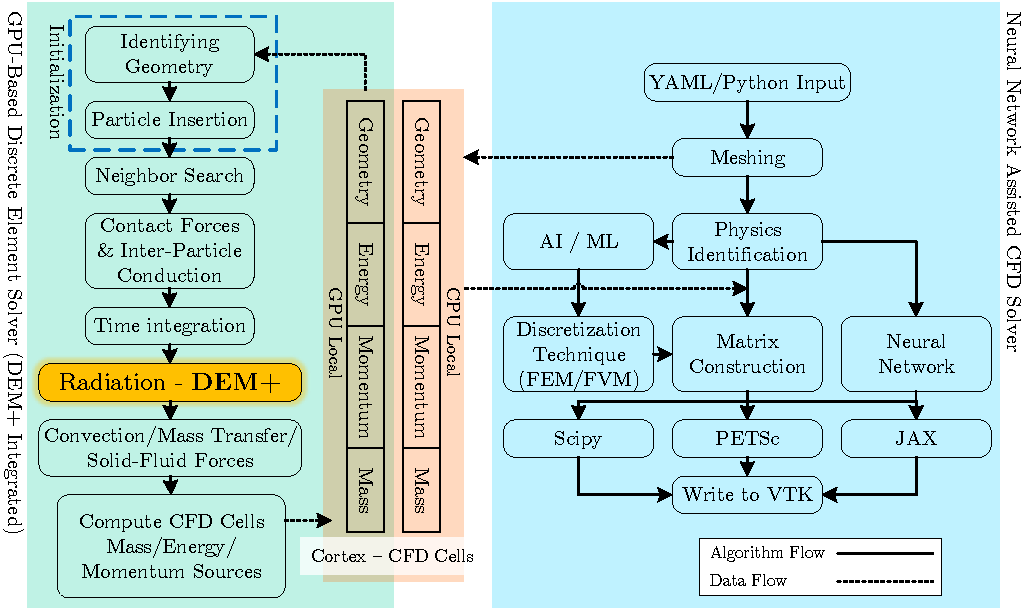
\includegraphics[width=0.8\textwidth]{figures/Flowchart.pdf}
\caption{Integration Flowchart: DEM+ provides radiative heating to GPU-DEM particles, which feed into FAME for ML-CFD analysis in the OSE.}
\label{fig:integration}
\end{figure}

\section*{Broader Impacts}
\vspace{-3pt}
\noindent
The FAME OSE ecosystem will democritize access to advanced thermal-fluid simulation and AI-assisted design tools across the manufacturing and energy sectors. A central aim is to train the next generation of researchers, engineers, and developers in open-source software development, digital twin technologies, and thermo-fluid modeling specific to manufacturing and energy. The project will offer annual hands-on workshops and summer schools focused on software sustainability and domain-specific applications. A targeted talent development initiative will engage institutions across various geographic regions through customized outreach and curriculum modules, helping to prepare a skilled, workforce-ready STEM pipeline. Research outcomes and practical use cases will be shared through peer-reviewed publications, conference tutorials, and freely accessible training materials hosted on the project's online platform and amplified through social media. By fostering a community grounded in open science, reproducibility, and collaborative development, this initiative will advance U.S. priorities in energy and manufacturing while ensuring the long-term sustainability of the FAME platform.

\section*{Risk Analysis/Security Plan}
\vspace{-3pt}
\noindent
This project identifies several key risks associated with transitioning FAME into an OSE, particularly those related to open-source products involving computational simulations and ML components. Primary risks include security vulnerabilities in the codebase that could lead to inaccurate thermal-fluid predictions, potentially compromising safety in AM processes (e.g., defect formation leading to structural failures in manufactured parts) or sCO$_2$ energy systems (e.g., inefficient heat transfer models). Data privacy concerns arise from handling experimental datasets, such as NIST AM benchmarks, which may contain sensitive material properties or proprietary process parameters. Ethical risks in AI/ML outputs include biases in the physics-guided heat source models, resulting in skewed surrogate predictions that disproportionately affect underrepresented applications in sustainable manufacturing. Additional risks encompass contributor attrition in the current small team, supply chain vulnerabilities from dependencies (e.g., PyTorch or NumPy libraries prone to unpatched exploits), and safety issues if collaboratively released artifacts enable misuse in high-stakes environments like aerospace certification.

To mitigate these, the project will follow CISA/NSA guidance on securing software supply chains, emphasizing secure-by-design principles such as integrating security early in development, conducting regular vulnerability management through automated scanning, and implementing identity and access controls to prevent unauthorized modifications \cite{souppayaSecureSoftwareDevelopment2022}. OpenSSF best practices will be adopted, including SLSA frameworks for ensuring supply chain integrity (e.g., verifiable builds and artifact provenance), security scorecards to assess project health, and standardized vulnerability disclosure policies \cite{SLSAOpenSource}. Specific strategies include establishing patching protocols (e.g., addressing known vulnerabilities within 30 days using tools like Dependabot), anonymizing datasets to comply with standards like GDPR or NIST privacy frameworks, and maintaining chain of custody via Git version control with signed commits. For ML-specific risks, bias audits will be incorporated to evaluate model fairness across diverse AM process parameters.

Phase I activities will explore mechanisms to ensure quality, secure modification, integration, and release of content. This includes conducting third-party security audits of the FAME codebase to identify baseline vulnerabilities, performing privacy impact assessments on sample datasets, and hosting workshops with experts to evaluate tools for identity and access management (e.g., GitHub's OAuth for contributor authentication). Exploration will also cover secure development methodologies, such as mandatory code reviews for pull requests and policies for patching dependencies, to build a robust foundation for collaborative OSE growth while addressing safety and privacy risks in released artifacts.
\vspace{-3pt}

\section*{Scoping Activities for Phase I}
\vspace{-3pt}
\noindent
Phase I scoping activities will focus on actionable planning to evaluate FAME's readiness for transition into a sustainable OSE, assess the viability of its emerging user base in AM and sCO$_2$ research communities, and identify a distributed developer community for ongoing maintenance and innovation. These activities are designed to be completed within the 1-year award period and \$300K budget, leveraging virtual tools, surveys, and targeted consultations to minimize costs while maximizing insights. Outputs will include a detailed roadmap for Phase II, such as drafted governance documents, community engagement strategies, and a prioritized list of ecosystem gaps. Activities will be coordinated by the PI team, with input from an external mentor experienced in open-source CFD ecosystems, and will incorporate feedback loops through quarterly progress reviews.

Specific scoping activities for Phase I include:
\vspace{-3pt}
\begin{itemize}
    \item \textbf{Ecosystem Discovery:} To evaluate the technological landscape, the team will conduct a comprehensive literature review and competitor analysis, surveying similar open-source CFD and ML tools (e.g., OpenFOAM for thermal-fluid simulations and PyTorch for ML integration). This will justify the need for FAME's innovation by highlighting gaps in physics-guided models for LPBF AM and sCO$_2$ systems, such as limited support for real-time optimization in proprietary alternatives. The OSE approach will be validated as ideal for distributed innovation, enabling asynchronous contributions unlike closed systems that restrict extensibility. Methods to identify potential users and developers include online surveys distributed to 50-100 stakeholders in AM/energy sectors (e.g., via professional networks like ASME and AIAA mailing lists) and analysis of GitHub metrics (e.g., forks, stars, and related repositories) to map interest from academia and industry.
    \item \textbf{Organization and Governance:} Activities will benchmark organizational models against established foundations (e.g., Apache Software Foundation for community-led governance or Linux Foundation for industry consortia) through case study reviews and consultations with 3-5 experts. Licensing options will be evaluated (e.g., MIT for permissiveness vs. GPL for copyleft protections) to ensure compatibility with ML dependencies like PyTorch. CI/CD infrastructure needs will be assessed, such as integrating GitHub Actions for automated testing on heterogeneous CPU/GPU setups to support asynchronous, distributed development. Processes for quality, security, privacy, and ethical concerns will be drafted, including guidelines for validating new ML models against NIST benchmarks. Sustainability methods will explore funding models (e.g., grants, donations via Open Collective) and metrics for long-term success, such as contributor retention rates $>$50\%, user support response times $<$48 hours, and onboarding completion rates measured via tutorial analytics.
    \item \textbf{Risk Analysis/Security:} Building on the dedicated risk plan, scoping tasks will include a third-party security audit of FAME's codebase using tools like SonarQube to baseline vulnerabilities, and privacy impact assessments on sample AM datasets to identify anonymization needs. Workshops (2 virtual sessions with 20-30 participants) will explore secure development practices, such as adopting OpenSSF scorecards for dependency management. Mechanisms for quality assurance (e.g., automated unit tests for thermal predictions), secure content integration (e.g., enforced code reviews via GitHub pull requests), identity and access management (e.g., OAuth for contributor authentication), and chain of custody (e.g., Git signed commits for provenance tracking) will be evaluated, with a focus on ML-specific risks like model bias through fairness audits.
    \item \textbf{Community Building:} To engage potential users and intellectual content developers, activities will identify required capabilities (e.g., proficiency in Python, CFD/ML for contributors; domain knowledge in AM/sCO$_2$ for users) via targeted surveys and interviews. Mechanisms include hosting 2-3 virtual workshops (e.g., introductory sessions on FAME's heat source modeling with 50+ participants from universities and labs) and a themed hackathon focused on extending FAME for sCO$_2$ applications. Online forums (e.g., GitHub Discussions) and research coordination networks (e.g., via Slack channels) will facilitate engagement. Inclusivity will be emphasized through scholarships for underrepresented participants (e.g., from HBCUs or women in STEM groups) and accessible materials, aiming to grow the contributor base from 2-3 to 10+ by project's end.
\end{itemize}

\section*{Community Outreach Plan}
\vspace{-3pt}
\noindent
The community outreach plan for the FAME OSE will proactively engage intellectual content developers (e.g., researchers and programmers in CFD and ML) to contribute to tool maintenance and extension, while identifying and onboarding user communities (e.g., AM and sCO$_2$ practitioners in academia, industry, and government labs) as early adopters. Drawing from best practices in open-source scientific software communities, such as those in OpenFOAM and PyTorch ecosystems, the plan emphasizes virtual, low-cost activities to build momentum within the 1-year Phase I timeframe, with a focus on inclusivity and measurable growth. All activities will be amplified through social media (e.g., LinkedIn, X/Twitter, and Reddit communities like r/AdditiveManufacturing and r/MachineLearning) and professional networks (e.g., ASME and AIAA forums) to reach diverse audiences.

To engage developers, quarterly webinars will cover contribution guidelines, FAME's modular architecture, and hands-on tutorials for extending ML models (e.g., integrating new heat source calibrations). An innovative virtual hackathon in Month 6 will challenge participants to develop FAME plugins for sCO$_2$ applications, using platforms like GitHub Classroom for collaborative coding and prizes sponsored by university partners. Developer onboarding will include mentorship pairings with the PI team, targeting 15-20 new contributors through targeted emails to CFD/ML mailing lists.

For identifying early adopters, initial surveys in Months 1-2 (distributed to 100+ stakeholders via email campaigns and conference booths at events like RAPID + TCT) will map user needs and potential adopters, such as small manufacturers lacking proprietary CFD tools. Partnerships will be forged with organizations like America Makes and NIST AM consortia through joint webinars and pilot use-case demonstrations, showcasing FAME's NIST-validated predictions. Social media campaigns will feature short video tutorials and case studies (e.g., AM defect reduction), aiming to convert viewers into beta testers.

Diversity and inclusion will be prioritized by collaborating with minority-serving institutions (e.g., HBCUs via the National Society of Black Engineers) and women-in-STEM groups (e.g., Society of Women Engineers), offering registration waivers and scholarships for events. Timelines include: Months 1-3 for surveys and initial webinars; Months 4-6 for hackathons and partnerships; Months 7-12 for follow-up evaluations and expanded outreach. Success will be tracked via engagement metrics (e.g., 200+ survey responses, 50+ webinar attendees), ensuring broad participation in advancing FAME's OSE.
\vspace{-3pt}

\section*{Evaluation Plan}
\vspace{-3pt}
\noindent
The evaluation plan for this Phase I project will employ actionable, quantitative, and qualitative metrics to assess progress toward scoping a sustainable OSE for FAME, focusing on product readiness, user base viability, and developer community potential. Drawing from metrics and indicators discussed in the Linux Foundation's report on open source for sustainability \cite{Sandberg2023}, including CHAOSS frameworks for community health and DEI, the plan integrates traditional tracking with novel approaches like AI-driven sentiment analysis on community feedback to provide dynamic insights. Evaluation will inform adaptive adjustments, ensuring alignment with NSF goals, and culminate in a Phase II readiness report. An external mentor will provide independent reviews, while the PI team conducts internal assessments.

Key metrics include: number of new contributors engaged (target: 10+ from baseline of 2-3, measured via GitHub commits and pull requests); user adoption growth (target: 50\% increase in downloads/stars, from current low baseline); completion of governance artifacts (e.g., 1 draft framework, 2-3 policy documents); community engagement levels (e.g., 100+ survey responses, 50+ event participants); and ecosystem health scores (e.g., CHAOSS-derived activity index >0.5, incorporating openness via license compatibility and scalability via modular extensions). Innovative metrics will track diversity in participation (e.g., 30\% from underrepresented groups, using self-reported demographics) and innovation impact (e.g., number of novel use cases proposed, assessed via hackathon outputs).

Assessment methods will combine repository analytics (e.g., GitHub Insights for contribution trends), pre/post-event surveys (e.g., Net Promoter Score for satisfaction), and automated tools like natural language processing for sentiment analysis on forum discussions and feedback forms to gauge inclusivity and ethical concerns. Quarterly reviews (Months 3, 6, 9, 12) will involve stakeholder meetings to analyze data, adjust activities (e.g., pivot outreach if engagement lags), and document lessons learned, ensuring transparent, data-driven progress toward OSE viability.
\vspace{-3pt}
\section*{Prior NSF Support}
\noindent
The PI's have no prior NSF support.
\newpage
\bibliographystyle{unsrt}
\bibliography{reference}
\end{document}